\documentclass[a4paper,11pt,oneside]{book}

\usepackage[english]{babel}
\usepackage[showframe=false]{geometry}
\usepackage[usenames,dvipsnames]{xcolor}
\usepackage[utf8]{inputenc}
\usepackage[T1]{fontenc}
\usepackage{changepage}
\usepackage[]{algorithm2e}
\usepackage{amssymb}
\usepackage{amsmath}
\usepackage{graphicx}
\usepackage{listings}
\usepackage{verbatimbox}
\usepackage{ulem}
\usepackage{fancyvrb}
\usepackage{float}
\usepackage{hyperref}
\usepackage[parfill]{parskip}
\usepackage{tikz}
\usepackage{pdflscape}
\usepackage{minted}
\usepackage{titlesec}
\usepackage{titleps}
\usepackage{lastpage}
\usepackage{fancyhdr}
\usepackage{etoolbox}
\usepackage[]{algorithm2e}
%Following overwrites the page style for chapters
\patchcmd{\chapter}{\thispagestyle{plain}}{\thispagestyle{ruledChapter}}{}{}

%New page style for chapters
\newpagestyle{ruledChapter}{
	\setfoot{}{\thepage\ of \pageref{LastPage}}{}
	\footrule
	\renewcommand\makefootrule{\color{black}\rule[\baselineskip]{\linewidth}{0.4pt}}
}
%New page style for rest
\newpagestyle{ruled}{
	\sethead{\raggedright \chaptername\ \thechapter :\ \chaptertitle}{}{}
	\headrule
	\setfoot{}{\thepage\ of \pageref{LastPage}}{}
	\footrule
	\renewcommand\makeheadrule{\color{black}\rule[-.3\baselineskip]{\linewidth}{0.4pt}}
	\renewcommand\makefootrule{\color{black}\rule[\baselineskip]{\linewidth}{0.4pt}}
}

\expandafter\def\csname PY@tok@err\endcsname{}
\newcommand{\HRule}{\rule{\linewidth}{0.5mm}}
\newcommand{\specialcell}[2][c]{%
  \begin{tabular}[#1]{@{}c@{}}#2\end{tabular}}

\addtocontents{toc}{\protect\thispagestyle{empty}}

\title{}
\author{}
\date{} 

\begin{document}
\begin{titlepage}
\begin{center}

%-----------------------------------------------------------------
%							FRONTPAGE
%-----------------------------------------------------------------
\thispagestyle{empty}

\includegraphics[width=0.55\textwidth]{logo.pdf}\\[1cm]    
\textsc{\Large DM818 Assignment 2}\\[0.5cm]

% Title
\begin{Huge}
\textbf{Parallelize Particle Simulation}
\end{Huge}

\vspace{4cm}

% Author and supervisor
\begin{minipage}{1\textwidth}
\begin{center}
\emph{}\\

Dan \textsc{Sebastian Thrane}\\
\verb!<dathr12@student.sdu.dk>!\\

Lars \textsc{Thomasen}\\
\verb!<latho12@student.sdu.dk>!\\

\end{center}
\end{minipage}
\begin{minipage}{0.4\textwidth}
\end{minipage}

\vfill

% Bottom of the page
{\large Winter 2015}\\

\end{center}
\end{titlepage}

%-----------------------------------------------------------------
%							   TOC
%-----------------------------------------------------------------
\renewcommand{\contentsname}{Table of Contents}
\tableofcontents
\thispagestyle{empty}

%-----------------------------------------------------------------
%						  ACTUAL REPORT
%-----------------------------------------------------------------
\pagestyle{ruled}
\chapter{Introduction}
\setcounter{section}{1}
This reports documents the second mandatory assignment for the course DM818 Parallel Computing. In this assignment we were given a particle simulation which runs in $O(n^{2})$ time, and were asked to code the following:

\begin{enumerate}
\item Change the implementation such that it runs in $O(n)$ time.
\item Parallelize the changed code using OpenMP/pThreads/MPI.
\end{enumerate}

In order to measure proper performance gain, we need to optimise the serial algorithm first, and then parallelize it such that the comparison stays fair. It would be easy to show a massive performance gain if the algorithm for the parallel implementation is vastly superior to the one used for linear.
 
\section{Work Load}
%A statement of who contributed with what.
The distribution of the workload has been equal, and pair programming in the imada terminal room have been the preferred method throughout this project.

\chapter{Making the implementation linear}
%A plot in log-log scale that shows that your serial and parallel codes run in O(n) time and a description of the data structures that you used to achieve it.
\section{The supplied algorithm}
The given algorithm for the serial implementation (and the parallel versions) are as follows, clearly running in $O(n^{2})$ runtime. This was unacceptable and thus a new algorithm has been developed.

\begin{verbatim}
for( int i = 0; i < n; i++ )
{
	particles[i].ax = particles[i].ay = 0;
	for (int j = 0; j < n; j++ )
	{
    	apply_force( particles[i], particles[j] );
    }
}
\end{verbatim}

The code above shows the culprit, when applying force to all particles, for each particle, all particles are iterated again to do so. Since a particle can only be influenced by nearby particles, this is extreme expensive.

\section{The new algorithm}
The range for interaction for the particles was reduced to a smaller value, denoted as the "cutoff" value. This cutoff value was showcased as a grey border on a particle in the assignment.

\begin{figure}[H]
  \centering
  \begin{minipage}[b]{0.4\textwidth}
    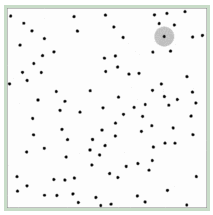
\includegraphics[width=\textwidth]{cutoff.png}
    \caption{Snapshot of the GIF from the assignment showcasing the influence ring.}
  \end{minipage}
\end{figure}

Having a reduced area of interaction, allows us to reduce the amount of particles influencing the amount of force needed to be applied to a given particle, thus we can reduce the second for-loop greatly.

In order to reduce the loop it is necessary to know which particles are within (or atleast close by) the particle we want to apply the force. To do this we needed to develop a data structure, to keep track of where the particles are positioned.

This data structure was not needed in the original solution since all particles were simply assumed to be within the cutoff range.

\section{The data structure}
In order to track the location of the particles, the coordinate system is divided into a grid, each coordinate holding all particles within a single cutoff range. It is then possible for a single particle, at a grid position, to find all particles in the surrounding grid positions, guaranteeing to find \emph{atleast} all particles within its cutoff range.

\begin{figure}[H]
  \centering
  \begin{minipage}[b]{0.4\textwidth}
    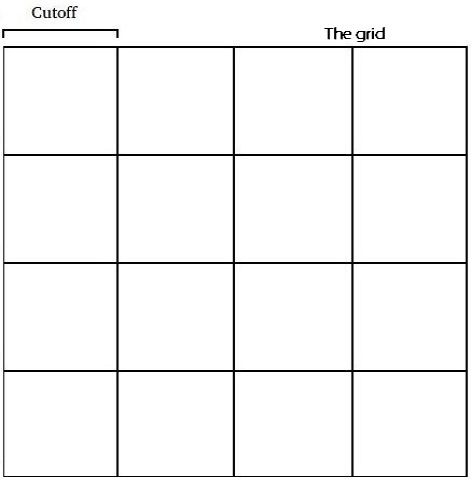
\includegraphics[width=\textwidth]{grid.jpg}
    \caption{The grid structure, showcasing the size of a single position equals the cutoff size.}
  \end{minipage}
  \begin{minipage}[b]{0.4\textwidth}
    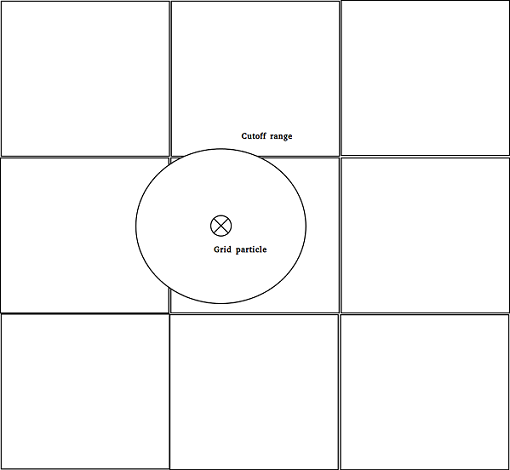
\includegraphics[width=\textwidth]{gridexample.png}
    \caption{A particle located inside a grid positions, and its influence range.}
  \end{minipage}
\end{figure}

Initially all particles are added to the data structure. It then has to be maintained whenever we move a particle, as the grid location could possibly change as the particle moves around.

\section{The implementation}
The implementation uses a separate file named \verb!grid.cpp! and \verb!grid.h!. These files holds the data structure and a series of helper methods that allows us to add, get and remove particles to the grid.

The grid itself is 	a vector of vectors with particles.

\begin{verbatim}
std::vector<std::vector<particle_t *> > grid;
\end{verbatim}

The coordinate positions consists of doubles, while the grid positions are mapped to integers. To overcome this the coordinate positions are simply converted using the following formulae, which simply moves the decimal two places to the right and casting to an integer. Thereby giving us a consistent mapping of doubles to integers:

\begin{align*}
\frac{\text{double value}}{0.01}
\end{align*}

Whenever we move a particle, we simply remove the particle from the grid completely, and then add it back in. This way the old position is removed, and the new position is calculated from the particles new position when added again. \\
This method assumes the particle always switches position in the grid, it could be calculated whether this actually is the case, but this was not done. Consequence to this method is that some unnecessary calculations might be performed whenever a particle do not move, since it would be removed and added back to the same grid position. The correctness of the algorithm is however not affected.

\section{The graphs}
Below is a graph plotted for different times (see appendix A) showcasing how the $O(n^{2})$ and $O(n)$ algorithms do versus each other. It is easy to see that the $O(n)$ is indeed linear. Note that bigger sizes did not terminate in reasonable time for the $O(n^{2})$ algorithm.

\begin{figure}[H]
  \centering
  \begin{minipage}[b]{0.9\textwidth}
    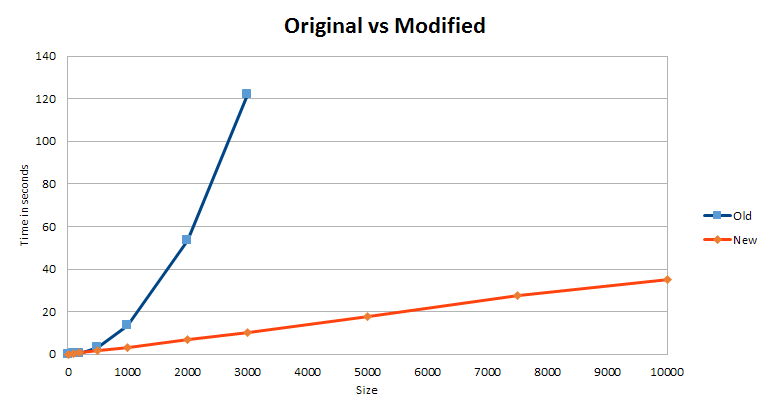
\includegraphics[width=\textwidth]{graph_regular.png}
    \caption{The original $O(n^{2})$ algorithm (blue) versus the new $O(n)$ algorithm (red).}
  \end{minipage}
\end{figure}


\chapter{Making the implementation parallel}
After having an optimal $O(n)$ running time for the serial implementation, the parallel algorithm can be developed. For this the MPI library was used.

\section{The algorithm}
% How was the linear algorithm modified to make it parallel.
In the parallel versions given in the assignment, each process is given and equal number of particles, and each process would then take its given particles and apply force to these against \emph{all} particles.


\IncMargin{1em}
\begin{algorithm}
\SetKwData{Left}{left}\SetKwData{This}{this}\SetKwData{Up}{up}
\SetKwFunction{Union}{Union}\SetKwFunction{FindCompress}{FindCompress}
\SetKwInOut{Input}{input}\SetKwInOut{Output}{output}
\Input{Local particles, All particles.}
\Output{Applied force to local particles.}
\BlankLine
\For{local particles i}{
\For{all particles j}{\label{forins}
apply force to i using j\;
}
}
\caption{Work each process does to particles.}\label{algo_disjdecomp}
\end{algorithm}\DecMargin{1em}

This will not work as it runs in $O(n^{2})$ and instead we need to use our grid implementation. This grid implementation will not be able to copy this approach as we need to know which particles are close to, or within the cutoff range.

The approach used here consists of splitting the grid evenly between processes, and then perform force to particles within each processes' own grid.

\subsection{Design choices}
%A description of the design choices that you tried and how did they affect the performance.
We wanted to reduce the overhead from communication as much as possibly, such that the idle time is as small as possible. In order to do this code complexity is compromised in that a lot of additional calculations have to be done, such that instead of communicating small bits of data often, each process instead calculates it instead.

\subsubsection{Ghost zones}


\subsubsection{Load balancing}
A situation may arise where all particles would cluster in one end of the grid, thus some processes would have a lot of work while some may have none. Load balancing would then divide the work from heavy loaded processes to those who have little work to do.

This is not handled in the implementation as it would add severe code complexity.

\section{The synchronization methods}
%A description of the synchronization you used in the shared memory implementation.
When processes need to communicate they often have to make sure they all are at the same instruction in the code. Therefore it is necessary to use different methods  to ensure that all processes are ready to exchange data.

\section{The communication}
%A description of the communication you used in the distributed memory implementation.
Communication arises between processes when a particle switches between grid borders between two processes.

\section{The graphs}
%Speedup plots that show how closely your parallel codes approach the idealized p-times speedup and a discussion on whether it is possible to do better.
%Where does the time go? Consider breaking down the runtime into computation time, synchronization time and/or communication time. How do they scale with p?

\chapter{Discussion on pthreads, OpenMP, and MPI}
%A discussion on using pthreads, OpenMP and MPI for this assignment.

\chapter{Conclusion}


%-----------------------------------------------------------------
%						     APPENDIX
%-----------------------------------------------------------------
\newpage
\newgeometry{left=2.5cm,right=2.5cm}
\chapter{Appendix}
\section{Serial algorithm plotting data}

\begin{figure}[H]
  \centering
  \begin{minipage}[b]{0.9\textwidth}
    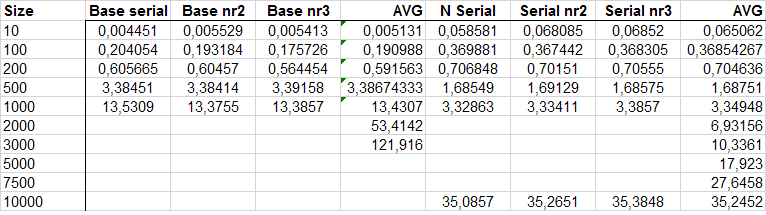
\includegraphics[width=\textwidth]{plotdata.png}
    \caption{Plotting data for the linear runtimes.}
  \end{minipage}
\end{figure}

\end{document}
